
%(BEGIN_QUESTION)


Regn ut differansetrykket som måles av DP-cellen ved tre forskjellige vannivåer i steam tanken. :0\%, 50\% og 100\%. 

$$\includegraphics[width=15.5cm]{i00516x01.eps}$$

Assume a density for (hot) boiler drum water of 36 lb/ft$^{3}$, a density for steam in the drum of 7 lb/ft$^{3}$, and a density for (warm) water in the ``wet leg'' of 61.8 lb/ft$^{3}$.  If the pressure at the ``low'' (L) side of the transmitter is greater than the pressure at the ``high'' (H) side, be sure to express the differential pressure quantity as a negative number.

\vskip 10pt

\noindent
Credit will be given for correctly calculating each of the differential pressures:

\begin{itemize}
\item{} {\bf (6 points)} Transmitter $\Delta$P at 0\% water level = \underbar{\hskip 50pt} "W.C.
\item{} {\bf (6 points)} Transmitter $\Delta$P at 50\% water level = \underbar{\hskip 50pt} "W.C.
\item{} {\bf (6 points)} Transmitter $\Delta$P at 100\% water level = \underbar{\hskip 50pt} "W.C.
\end{itemize}

\underbar{file i00516}
%(END_QUESTION)





%(BEGIN_ANSWER)

\begin{itemize}
\item{} {\bf (6 points)} Transmitter $\Delta$P at 0\% water level = \underbar{\bf -38.832} "W.C.
\item{} {\bf (6 points)} Transmitter $\Delta$P at 50\% water level = \underbar{\bf -31.864} "W.C.
\item{} {\bf (6 points)} Transmitter $\Delta$P at 100\% water level = \underbar{\bf -24.896} "W.C.
\end{itemize}

%(END_ANSWER)





%(BEGIN_NOTES)


%INDEX% Measurement, level: hydrostatic pressure (suppressed zero)

%(END_NOTES)


